\section{Server Backend}
This chapter covers the core component of the iCare Server: The Server Backend. The following subchapters describe the architecture of the server with its individual components and the technologies used to implement communication between the subsystems.
\subsection{The Server architecture}
The following figure \ref{icare-serverarchitecure} shows the general architecture of the backend server and the external systems with which the server communicates at runtime. The focus here lies on the \textit{iCare Server} subsystem, while the other components of the system \textit{iCare Frontend}, \textit{iCare Room HUB}, \textit{iCare Backup System} and \textit{iCare Data} are treated as black boxes. 
\begin{figure}[H]
	\centering
	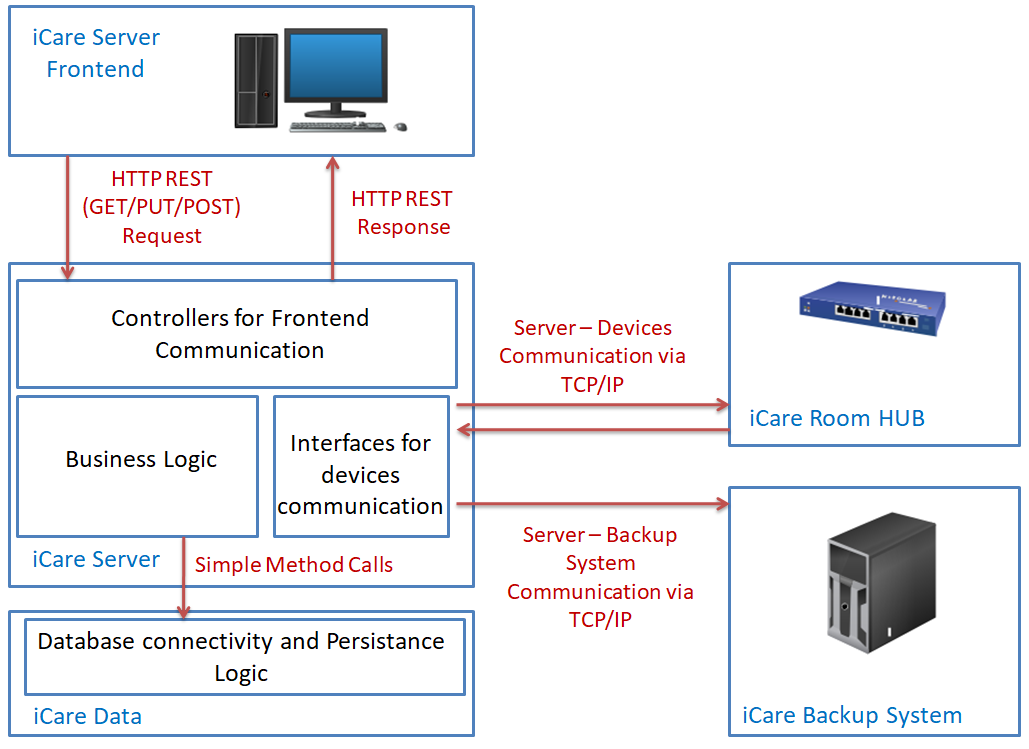
\includegraphics[width =1.0\textwidth]{images/server-architecture.PNG}
	\caption{iCare Server architecture}
	\label{icare-serverarchitecure}
\end{figure}
As can be seen in the picture, the iCare web server has communication interfaces to the other subsystems, which are based on different technologies. The communication between the frontend and the backend is based on Representational State Transfer (REST) web services. The communication with the different devices, which are accessible via a network hub in the individual rooms, works with simple Java sockets. Because the iCare Data module runs on the same system, there is a direct dependency relationship between the iCare Data module and the iCare Server module, enabling the web server to directly access the interfaces of the iCare Data module.
\subsection{Communication between frontend and backend via REST}
As already mentioned, the communication between frontend and backend works via RESTful web services. The web server provides controller classes as access points for the requests of the iCare frontend, which can be reached at the host address of the web server under corresponding extensions. The following address is an example for this kind of access point.
\begin{center}
	\textit{http://www.iCareWeb.de:8080/inhabitant}
\end{center}
The \textit{/inhabitant} access point for example provides a list of all care home residents that carry a wrist band and the corresponding data captured by the wrist band in real time. For example, if the frontend is to display this data in a user interface, a GET request must only be sent to this endpoint at regular intervals. As a response, the frontend receives the current data of all wrist bands packed in a JSON string. The following listing shows one entry in this JSON-String:
\begin{lstlisting}
{
	"id": "a64f3d5c-bade-49f8-b67f-2d5b7d0c55a5",
	"heartRate": 55,
	"name": "Ms. Smith",
	"restrictions": [],
	"healthCheck": {
		"message": "Low heart rate",
		"status": "YELLOW"
	},
	"position": {
		"x": 29,
		"y": 33
	}
}
\end{lstlisting}
How this JSON string is interpreted and displayed lies with the frontend and is not discussed here any further.
\\
The functions for controlling the central heating system can also be called via PUT and POST requests. To do this, a similar JSON string must be packed into the request, which contains the required data. The server then interprets this JSON string and executes the command for the corresponding radiator in the specified room.

\subsection{Communication between Server and Devices/Backup system}
\subsection{Business Logic}
\subsection{Connection to ICare Data}